\chapter{THIẾT KẾ HỆ THỐNG}

\section{Thiết kế Kiến trúc (Architecture Design)}
Để đảm bảo hệ thống có khả năng bảo trì cao, dễ dàng mở rộng và độc lập với các thư viện hoặc cơ sở dữ liệu, dự án được xây dựng dựa trên nguyên lý của mô hình \textbf{Clean Architecture} \cite{cleanarchitecture}. Mã nguồn Backend chia thành 4 project (4 tầng đồng tâm):

\begin{enumerate}
    \item \textbf{CloudService.Domain (Core):} Chứa các logic nghiệp vụ cốt lõi, hoàn toàn thuần C\#. Gồm 9 thực thể (Entities), 3 Enums (\texttt{UserRole}, \texttt{OrderStatus}, \texttt{BillingCycle}), lớp cơ sở \texttt{BaseEntity} và các giao diện Repository. Lớp này \textbf{không tham chiếu} đến bất kỳ lớp nào khác.
    \item \textbf{CloudService.Application:} Đóng vai trò làm lớp trung gian (Use Cases), chứa 8 Services (\texttt{OrderService}, \texttt{CategoryService}, \texttt{NewsArticleService}, \texttt{ServicePlanService}, \texttt{AffiliateService}, \texttt{AuditLogService}, \texttt{AuthService}, \texttt{AdminStatsService}) cùng 9 giao diện (Interfaces) tương ứng và các DTOs (Data Transfer Objects).
    \item \textbf{CloudService.Infrastructure:} Thực thi (Implement) các giao diện được định nghĩa ở lớp Core. Chứa: \texttt{AppDbContext} (DbContext của EF Core), 7 Repository cụ thể, lớp \texttt{UnitOfWork}, và 5 Infrastructure Services (\texttt{JwtService}, \texttt{PasswordHashService}, \texttt{QrCodeService}, \texttt{ExcelExportService}, \texttt{AuthService}).
    \item \textbf{CloudService.WebApi (Presentation):} Là lớp giao tiếp với bên ngoài (Frontend). Chứa 14 Controllers (5 Public + 9 Admin), 2 Middleware (\texttt{ExceptionMiddleware}, \texttt{AuditMiddleware}) và cấu hình Dependency Injection tại \texttt{Program.cs}.
\end{enumerate}

% TODO: Chèn ảnh Sơ đồ kiến trúc hệ thống. Hãy lưu file ảnh tên là 'clean_architecture.png' vào thư mục 'images'
\begin{figure}[htbp]
    \centering
    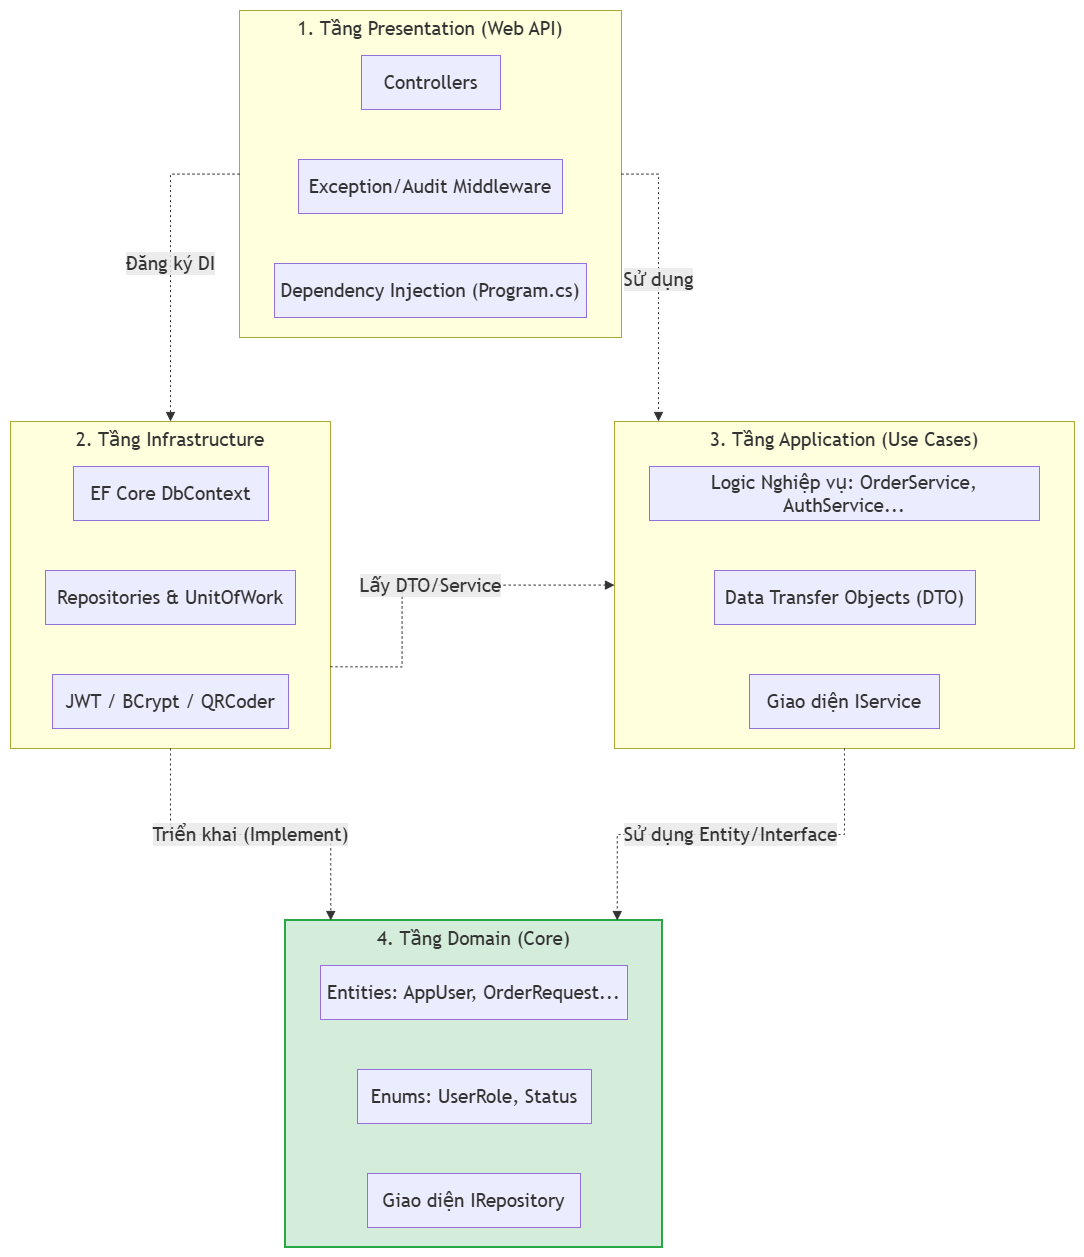
\includegraphics[width=0.9\textwidth]{images/clean_architecture.png}
    \caption{Sơ đồ khối Clean Architecture trong dự án}
    \label{fig:clean_arch}
\end{figure}

\section{Thiết kế Cơ sở dữ liệu (Database Design)}
Dữ liệu của hệ thống được thiết kế chặt chẽ và chuẩn hóa nhằm tránh dư thừa thông tin. Hệ thống sử dụng tổng cộng \textbf{10 bảng} (tương ứng 9 Entities + 1 bảng Role tích hợp Enum).

\subsection{Sơ đồ thực thể liên kết (ERD)}
% TODO: Chèn ảnh Sơ đồ ERD. Hãy lưu file ảnh tên là 'erd.png' vào thư mục 'images'
\begin{figure}[htbp]
    \centering
    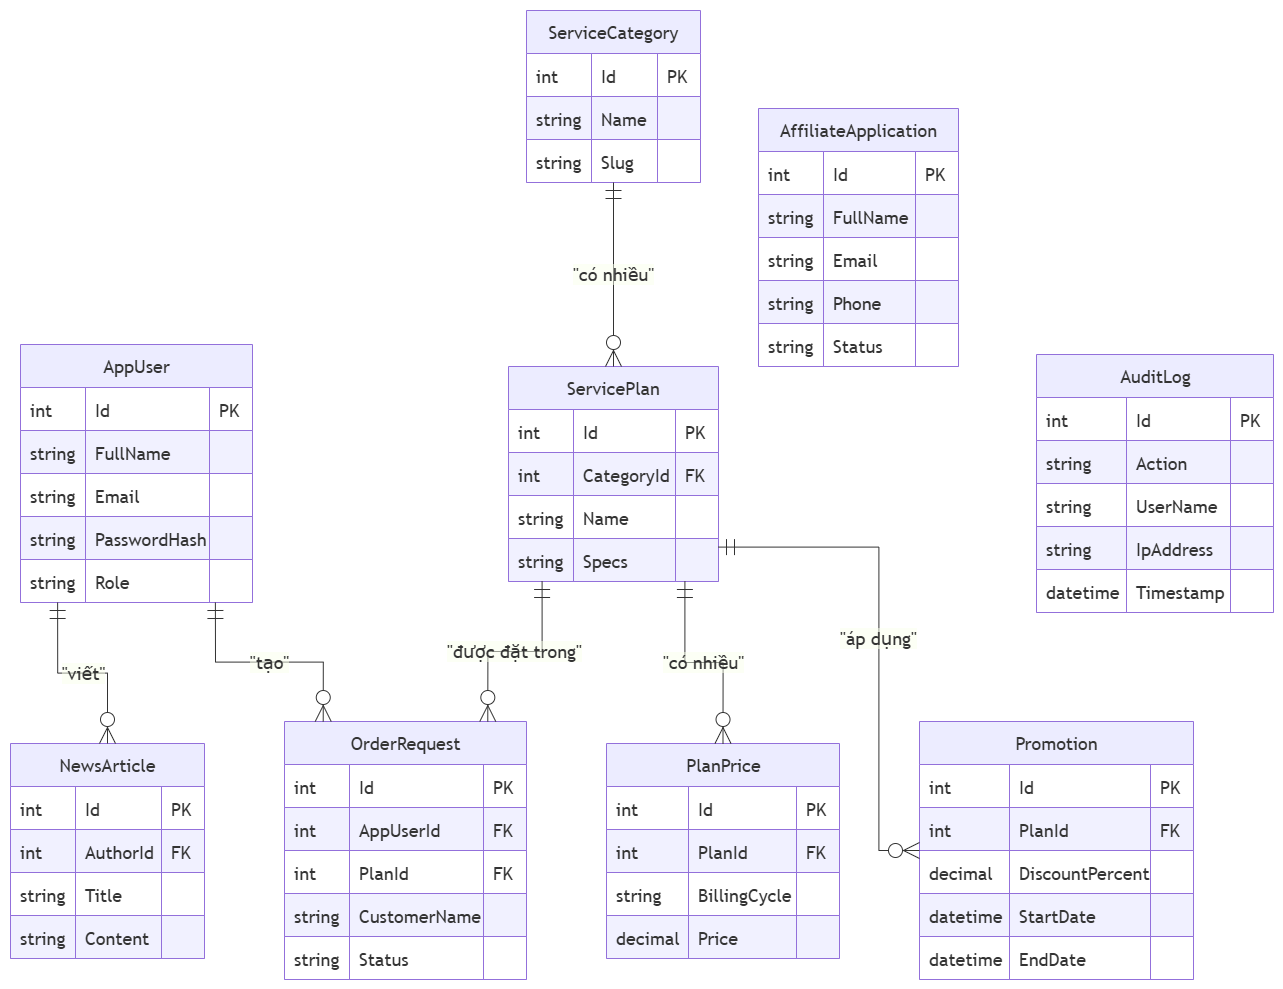
\includegraphics[width=1\textwidth]{images/erd.png}
    \caption{Sơ đồ thực thể liên kết (ERD)}
    \label{fig:erd}
\end{figure}

\subsection{Mô tả các thực thể (Entities) chính}
Bảng~\ref{tab:entities} mô tả chi tiết 9 thực thể chính được triển khai trong hệ thống, tất cả đều kế thừa từ \texttt{BaseEntity} (chứa \texttt{Id}, \texttt{CreatedAt}, \texttt{UpdatedAt}).

\begin{table}[htbp]
    \centering
    \caption{Danh sách các thực thể (Entities) trong hệ thống}
    \label{tab:entities}
    \begin{tabular}{|c|p{3.5cm}|p{8.5cm}|}
        \hline
        \textbf{STT} & \textbf{Entity} & \textbf{Mô tả và các thuộc tính chính} \\
        \hline
        1 & \texttt{ServiceCategory} & Danh mục dịch vụ gốc (VPS, Hosting, Domain). Thuộc tính: \texttt{Name}, \texttt{Slug}, \texttt{Description}. Quan hệ 1-N với \texttt{ServicePlan}. \\
        \hline
        2 & \texttt{ServicePlan} & Gói dịch vụ cụ thể. Thuộc tính: \texttt{Name}, \texttt{Slug}, \texttt{Specs} (CPU/RAM/SSD), \texttt{CategoryId}. Quan hệ N-1 với \texttt{ServiceCategory}, 1-N với \texttt{PlanPrice}. \\
        \hline
        3 & \texttt{PlanPrice} & Bảng giá theo chu kỳ. Thuộc tính: \texttt{BillingCycle} (Monthly/Yearly), \texttt{Price}, \texttt{PlanId}. Cho phép một gói có nhiều mức giá khác nhau. \\
        \hline
        4 & \texttt{Promotion} & Chương trình khuyến mãi. Thuộc tính: \texttt{PlanId}, \texttt{DiscountPercent}, \texttt{StartDate}, \texttt{EndDate}, \texttt{IsActive}. Quan hệ N-1 với \texttt{ServicePlan}. \\
        \hline
        5 & \texttt{NewsArticle} & Bài viết/Tin tức. Thuộc tính: \texttt{Title}, \texttt{Slug}, \texttt{Content} (HTML), \texttt{Summary}, \texttt{Category}, \texttt{AuthorId}. \\
        \hline
        6 & \texttt{OrderRequest} & Yêu cầu đặt dịch vụ. Thuộc tính: \texttt{CustomerName}, \texttt{Email}, \texttt{Phone}, \texttt{ServiceName}, \texttt{PlanId}, \texttt{BillingCycle}, \texttt{Status} (Enum: Pending/Processing/Completed/Rejected). \\
        \hline
        7 & \texttt{AffiliateApplication} & Đơn đăng ký đối tác. Thuộc tính: \texttt{FullName}, \texttt{Email}, \texttt{Phone}, \texttt{Website}, \texttt{Status}. \\
        \hline
        8 & \texttt{AppUser} & Tài khoản quản trị. Thuộc tính: \texttt{FullName}, \texttt{Email}, \texttt{PasswordHash}, \texttt{Role} (Enum: Admin/Editor), \texttt{RefreshToken}, \texttt{RefreshTokenExpiry}. \\
        \hline
        9 & \texttt{AuditLog} & Nhật ký hệ thống. Thuộc tính: \texttt{Action}, \texttt{UserName}, \texttt{IpAddress}, \texttt{Timestamp}, \texttt{Details}. \\
        \hline
    \end{tabular}
\end{table}

\section{Thiết kế RESTful API}
Backend cung cấp tổng cộng \textbf{37 endpoints} chia thành 3 nhóm chính. Bảng~\ref{tab:api_endpoints} liệt kê các endpoint tiêu biểu.

\begin{table}[htbp]
    \centering
    \caption{Danh sách các API Endpoint chính}
    \label{tab:api_endpoints}
    \begin{tabular}{|p{1.5cm}|p{5.5cm}|p{5cm}|}
        \hline
        \textbf{Method} & \textbf{Route} & \textbf{Mô tả} \\
        \hline
        \multicolumn{3}{|c|}{\textit{Public API (Không cần đăng nhập)}} \\
        \hline
        GET & \texttt{/api/public/service-categories} & Danh mục dịch vụ \\
        GET & \texttt{/api/public/service-plans} & Tất cả gói dịch vụ \\
        GET & \texttt{/api/public/service-plans/\{id\}/qr} & Mã QR cho gói DV \\
        GET & \texttt{/api/public/news} & Danh sách tin tức \\
        GET & \texttt{/api/public/news/\{slug\}} & Chi tiết bài viết \\
        POST & \texttt{/api/public/orders} & Gửi yêu cầu đặt DV \\
        POST & \texttt{/api/public/affiliates} & Đăng ký affiliate \\
        \hline
        \multicolumn{3}{|c|}{\textit{Auth API}} \\
        \hline
        POST & \texttt{/api/auth/login} & Đăng nhập $\rightarrow$ JWT \\
        POST & \texttt{/api/auth/refresh} & Gia hạn Access Token \\
        POST & \texttt{/api/auth/change-password} & Đổi mật khẩu \\
        \hline
        \multicolumn{3}{|c|}{\textit{Admin API (Yêu cầu JWT + Role)}} \\
        \hline
        CRUD & \texttt{/api/admin/service-plans} & Quản lý gói DV \\
        CRUD & \texttt{/api/admin/categories} & Quản lý danh mục \\
        CRUD & \texttt{/api/admin/news} & Quản lý tin tức \\
        CRUD & \texttt{/api/admin/promotions} & Quản lý khuyến mãi \\
        GET & \texttt{/api/admin/stats/summary} & Thống kê tổng quan \\
        GET & \texttt{/api/admin/export/orders} & Xuất Excel đơn hàng \\
        GET & \texttt{/api/admin/audit-logs} & Nhật ký hệ thống \\
        \hline
    \end{tabular}
\end{table}

\section{Thiết kế Mẫu thiết kế (Design Patterns)}
Các mẫu thiết kế (Design Patterns) \cite{gof} là những giải pháp tối ưu đã được kiểm chứng cho các vấn đề lặp lại trong thiết kế phần mềm. Dự án áp dụng các pattern sau:

\subsection{Repository Pattern}
Lớp \texttt{IGenericRepository<T>} cung cấp một tập hợp các hàm CRUD tiêu chuẩn chung cho mọi bảng. Các lớp nghiệp vụ chỉ cần gọi các phương thức như \texttt{GetAllAsync}, \texttt{GetByIdAsync} mà không cần biết chi tiết về câu lệnh SQL dưới tầng hạ tầng. Điều này giúp mã nguồn Application hoàn toàn không bị ``trói buộc'' với Entity Framework.

Trong dự án, 7 Repository cụ thể đã được triển khai: \texttt{ServiceCategoryRepository}, \texttt{ServicePlanRepository}, \texttt{NewsArticleRepository}, \texttt{OrderRequestRepository}, \texttt{AffiliateApplicationRepository}, \texttt{AppUserRepository}, \texttt{AuditLogRepository}.

\subsection{Unit of Work Pattern}
Khi có nhiều Repositories cần tương tác với Database cùng một lúc (ví dụ: tạo đơn hàng \texttt{OrderRequest} và cập nhật trạng thái affiliate), mô hình Unit of Work (giao diện \texttt{IUnitOfWork}) được sử dụng để gom các thao tác này vào chung một Giao dịch (Transaction). Lệnh \texttt{CompleteAsync()} đảm bảo dữ liệu chỉ được lưu nếu không xảy ra lỗi.

\subsection{Middleware Pattern}
Hệ thống sử dụng 2 Middleware tùy chỉnh theo dạng ``ống nước'' (Pipeline):
\begin{itemize}
    \item \texttt{ExceptionMiddleware}: Bắt toàn bộ exception chưa được xử lý và trả về response JSON chuẩn với mã lỗi HTTP phù hợp (400, 404, 500).
    \item \texttt{AuditMiddleware}: Tự động ghi lại mọi hành động quan trọng (đăng nhập, thay đổi dữ liệu) vào bảng \texttt{AuditLog} kèm thông tin IP, thời gian và người thực hiện.
\end{itemize}

\subsection{Dependency Injection (DI)}
Toàn bộ việc ``nối dây'' giữa các Interface và Implementation được cấu hình tập trung tại \texttt{Program.cs} thông qua DI container tích hợp sẵn của ASP.NET Core. Ví dụ:

\begin{verbatim}
builder.Services.AddScoped<IOrderService, OrderService>();
builder.Services.AddScoped<ICategoryService, CategoryService>();
builder.Services.AddScoped<IUnitOfWork, UnitOfWork>();
\end{verbatim}

\section{Sơ đồ Tuần tự (Sequence Diagram)}
Sơ đồ tuần tự thể hiện sự giao tiếp và thứ tự các thông điệp truyền đi giữa Client (Frontend) và Server (Backend) trong một chức năng. 

Dưới đây minh họa quy trình Đăng nhập và nhận JWT Token: Frontend gửi \texttt{POST /api/auth/login} $\rightarrow$ AuthController gọi AuthService $\rightarrow$ kiểm tra PasswordHash bằng BCrypt $\rightarrow$ JwtService sinh AccessToken + RefreshToken $\rightarrow$ trả về Frontend lưu Cookie.

% TODO: Chèn ảnh Sơ đồ Tuần tự quá trình Đăng nhập. Hãy lưu file ảnh tên là 'sequence_login.png' vào thư mục 'images'
\begin{figure}[htbp]
    \centering
    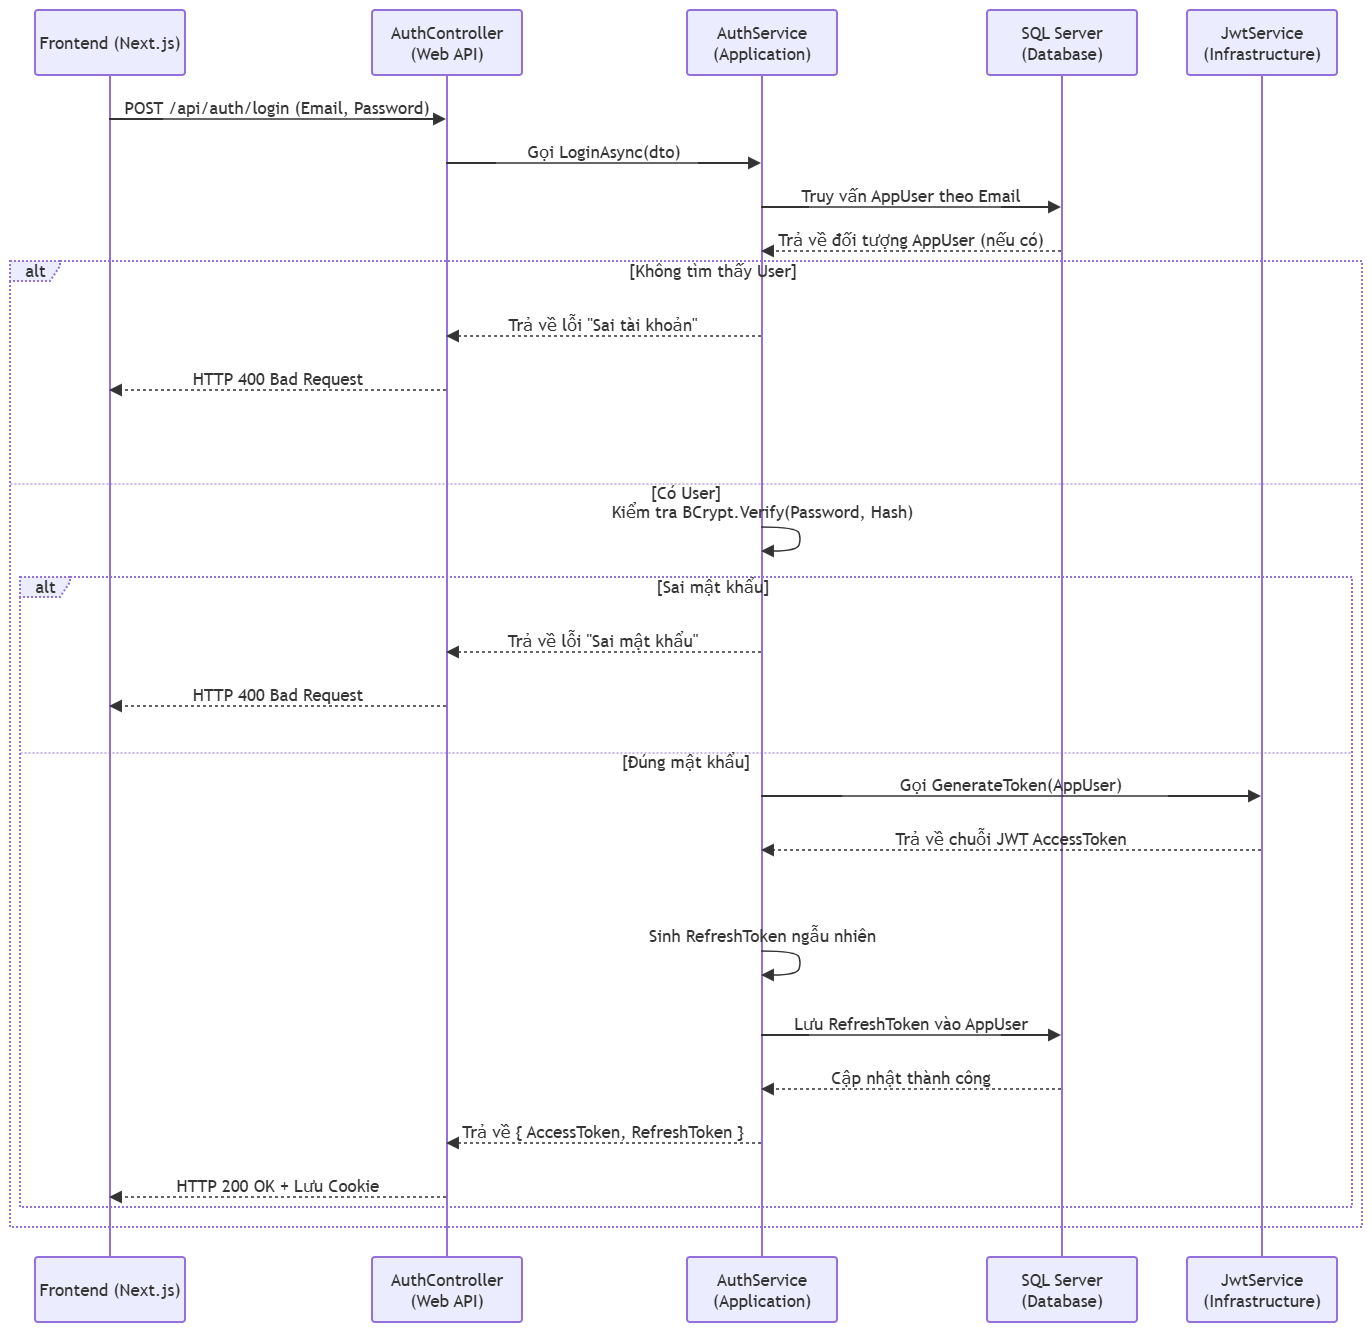
\includegraphics[width=0.9\textwidth]{images/sequence_login.png}
    \caption{Sơ đồ Tuần tự luồng xử lý xác thực đăng nhập cấp phát JWT}
    \label{fig:sequence_login}
\end{figure}
